\documentclass[a4paper]{article}
\usepackage[utf8]{inputenc}
\usepackage[french]{babel}
\usepackage[T1]{fontenc}
\usepackage{lmodern}
\usepackage[left=2cm,right=2cm,top=2cm,bottom=2cm]{geometry}
\usepackage{graphicx}
\usepackage{subfigure}
\usepackage{enumitem}
\usepackage{stmaryrd}
\usepackage{amsmath}
\usepackage{amssymb}
\usepackage{amsthm}
\usepackage{multicol}
\usepackage{hyperref}
\hypersetup{hidelinks}
\usepackage{color}
\usepackage{pdfpages}
\usepackage{ebproof}


\newcommand{\N}{\ensuremath{\mathbb{N}}}
\newcommand{\Z}{\ensuremath{\mathbb{Z}}}
\newcommand{\Q}{\ensuremath{\mathbb{Q}}}
\newcommand{\znz}{\ensuremath{\mathbb{Z} / n \mathbb{Z}}}
\newcommand{\G}{\Gamma}
\DeclareMathOperator{\fv}{\mathrm{fv}}
\DeclareMathOperator{\bv}{\mathrm{bv}}
\renewcommand{\epsilon}{\varepsilon}
\renewcommand{\leq}{\leqslant}
\renewcommand{\geq}{\geqslant}
\newcommand{\defi}{\overset{\text{def}}{=}}
\newcommand{\PA}{\mathsf{PA}}
\newcommand{\HA}{\mathsf{HA}}
\newcommand{\ZF}{\mathsf{ZF}}
\newcommand{\NJ}{\mathsf{NJ}_1}
\newcommand{\NK}{\mathsf{NK}_1}


\newcommand{\fonc}[5]{#1 : 
\left|
\begin{array}{ccc}
#2 & \longrightarrow & #3 \\
#4 & \longmapsto & #5
\end{array}
\right.
}

\newtheorem{theorem}{Théorème}[section]
\newtheorem{coro}{Corollaire}[theorem]
\newtheorem{lemma}[theorem]{Lemme}
\newtheorem{prop}[theorem]{Proposition}
\theoremstyle{remark}
\newtheorem*{rmq}{Remarque}
\theoremstyle{remark}
\newtheorem*{notation}{Notation}
\theoremstyle{remark}
\newtheorem{exemple}{Exemple}[section]
\theoremstyle{definition}
\newtheorem{df}[theorem]{Définition}
\theoremstyle{definition}
\newtheorem{algo}[theorem]{Algorithme}
\theoremstyle{definition}
\newtheorem{pb}[theorem]{Problème}

\usepackage{titlesec}
\titleformat*{\section}{\bf\Large\sffamily}
\titleformat*{\subsection}{\bf\large\sffamily}
\titleformat*{\subsubsection}{\bf\sffamily}

\title{Extensions d'un cours de logique du premier ordre certifié en Coq}
\author{Samuel Ben Hamou}
\date{\today}

\begin{document}
\begin{center}
    \vspace*{4em}
    {\LARGE Rapport de stage} \\ \vspace{1em}
    {\huge Extensions d'un cours de logique du premier ordre certifié en Coq} \\ \vspace{2em}
    
    {\Large Stage effectué du 1 juin au 17 juillet 2020} \\ \vspace{3em}
    
    {\Large Samuel Ben Hamou} \\
    {\large \'Ecole Normale Supérieure Paris-Saclay} \\ 
    {\large 1ère année, département informatique} \\ \vspace{2em}
    
    {\Large Sous la supervision de Pierre Letouzey} \\
    {\large IRIF, INRIA et CNRS} \vspace{2em}
\end{center}


\begin{abstract}
Ce stage de recherche de fin de licence avait pour but de proposer des extensions à un encodage en Coq déjà existant de la déduction naturelle. Le dépôt du projet se trouve à l'adresse suivante : \url{https://gitlab.math.univ-paris-diderot.fr/letouzey/natded}.

Dans un premier temps, il a fallu se familiariser avec les outils du stage : à la fois la manipulation de Git mais aussi l'encodage parfois étonnant des notions classiques de la logique (formules closes, variables liées, modèles, etc.). Un fois ce travail de défrichage effectué, nous avons pu enrichir le codage existant en suivant trois axes principaux, qui correspondent aux trois sections principales de ce rapport :
\begin{itemize}
\item l'arithmétique de Peano, qui avait déjà été encodée mais où tout restait à faire du point de vue des exemples et de la maniabilité des preuves,
\item la théorie des ensembles $\ZF$, où il s'est agit non seulement d'encoder les axiomes et de faire quelques preuves exemples, mais aussi de montrer qu'elle était plus générale que $\PA$, en ce sens qu'on peut démontrer dans $\ZF$ l'ensemble des axiomes de $\PA$. En pratique, il n'a pas été démontré exactement $\ZF \vdash \PA$, par manque de temps, mais on a défini dans $\ZF$ des fonctions zéro et successeur, qui servent de base à l'arithmétique de Peano.
\item le $\lambda$-calcul enfin
\end{itemize}
\end{abstract}

\renewcommand{\contentsname}{\centerline{Table des matières} \vspace*{-2em}}
\tableofcontents

\newpage

\section{Introduction}

\subsection{Contexte pratique du stage}

Ce stage a été effectué sous la direction de Pierre Letouzey, maître de conférence à l'Université Paris-Diderot, et membre du groupe $\pi r^2$ de l'IRIF. Compte tenu du contexte sanitaire, la majeur partie des échange a eu lieu via BBB et par mail, à un rythme assez soutenu. J'ai cependant pu me rendre physiquement à l'IRIF afin de discuter dans la vraie vie avec avec mon maître de stage.

Malgré les échanges de mails réguliers, le travail à distance a probablement été le plus gros inconvénient de ce stage : dans la mesure où je travaillais sur un codage créé par Pierre Letouzey, qui n'a pas écrit de manuel d'explication pour justifier ou expliquer ses choix d'implémentation (ce qui se conçoit parfaitement étant donné l'usage qu'il avait prévu de faire de son travail, qui n'était censé être utilisé que pour illustrer le cours de logique qu'il donne en M1), j'ai dans eu grandement besoin d'explications pour me lancer dans le travail, et il eût probablement été plus aisé d'avoir ce genre de discussions informelles si nous avions pu travailler dans deux bureaux adjacents.

Il n'en demeure pas moins que le stage a pu se dérouler sans trop d'embuche, et sans problèmes matériels majeurs. Par ailleurs, le travail à distance présente l'avantage non négligeable de permettre à chacun de travailler aux horaires qui lui conviennent le mieux, fût-ce tard le soir (ou bien tôt le matin selon la façon dont on voit les choses).

\subsection{Motivations}

Le but du stage a été d'enrichir l'encodage de \verb+NatDed+ déjà existant, tout en gardant en tête la vocation pédagogique du projet, puisqu'il s'agit d'illustrer un cours de logique de M1 \cite{poly}.

\verb+NatDed+ étant à l'origine assez rustique, il était pédagogiquement intéressant de le rendre plus \textit{user-friendly}, mais aussi d'ajouter un certain nombre d'exemples et d'applications (la théorie $\ZF$ par exemple), qui manquaient au projet initial.

Par la suite, il a été à propos d'ajouter d'autres aspects de la logique à cet encodage, tels que le $\lambda$-calcul, la théorie des ensembles et éventuellement la logique intuitionniste (en particulier les modèles de Kripke), qui sont tous des point abordés dans le cours donné par Pierre Letouzey. En effet, le $\lambda$-calcul est un élément essentiel de la construction des assistants de preuve tels que Coq.

\subsection{Encodage existant et état de l'art}

% système de déduction naturelle présent (avec séquents et en coq)
% distinction pr ou valid
% locally nameless

\subsection{Mise en place de l'environnement de travail}

Avant de se lancer dans le stage à proprement parler, il a fallu consacrer une petite semaine à l'acquisition de réflexes de travail, à la fois sur le support (GitHub) et sur l'encodage lui-même.

\subsubsection{Dépôt Git}

La première journée du stage a été passée à appréhender un outil nouveau pour manipuler de gros projets de code : GitHub. \'A ce titre, et pour me fixer les idées, j'ai rédigé la cheatsheet présentée en \ref{gitsheet}.

L'usage de Git a été d'un grand recours, notamment lorsque nous voulions discuter d'un morceau de preuve en visio-conférence, car chacun pouvait travailler et mettre à jour le dépôt de son côté, la fusion se faisant ensuite aisément grâce à la commande \verb+git pull+.

\subsubsection{Premières preuves}

Afin de me faire la main sur un encodage déjà très évolué, j'ai tenté de démontrer les petits résultats classiques suivants :
\begin{itemize}
\item $\vdash (\phi_1 \wedge \phi_2) \Rightarrow (\phi_1 \vee \phi_2)$,
\item $\vdash (\phi_1 \Rightarrow \phi_2 \Rightarrow \phi_3) \Leftrightarrow (\phi_1 \wedge \phi_2 \Rightarrow \phi_3)$,
\item $\vdash \phi \vee \neg \phi$.
\end{itemize}
Pour ce dernier point, il a été utile d'établir l'admissibilité des règles suivantes : \[ \begin{prooftree}
\hypo{\Gamma \vdash \neg \neg \phi}
\infer1[RAA]{\Gamma \vdash \phi}
\end{prooftree} \qquad \begin{prooftree}
\hypo{\Gamma \vdash \neg (\neg \phi_1 \wedge \phi_2)}
\infer1[Morgan]{\Gamma \vdash \phi_1 \vee \neg \phi_2}
\end{prooftree} \] puisque la règle de l'absurde présente dans l'encodage initial était \begin{prooftree*}
\hypo{\neg \phi, \Gamma \vdash \bot}
\infer1[absu]{\Gamma \vdash \phi}
\end{prooftree*}
\'Evidemment, les règles RAA et absu sont équivalentes, mais la forme RAA était plus commode pour montrer le tiers-exclu.

% Comment présenter du verbatim coq ? faut-il le faire ici ? -> Oui
% DIRE QUE L'ON A UTILISE DU SUCRE SYNTAXIQUE
% alltt ?


\section{Arithmétique de Peano}

\subsection{Constats de départ}

\subsection{Définition de nouvelles tactiques}


\section{Théorie des ensembles de Zermelo-Fraenkel}

\subsection{Encodage des axiomes et méta-théorèmes}

\subsection{Preuves exemples}

\subsection{Autour de $\ZF \vdash \PA$}


\section{Lien avec le $\lambda$-calcul}


\section{Conclusion}

\bibliographystyle{plain}
%\renewcommand{\refname}{Bibliographie}
\nocite{*}
\bibliography{biblio}

\appendix
\newpage

\section{Définition de \texttt{Pr}}

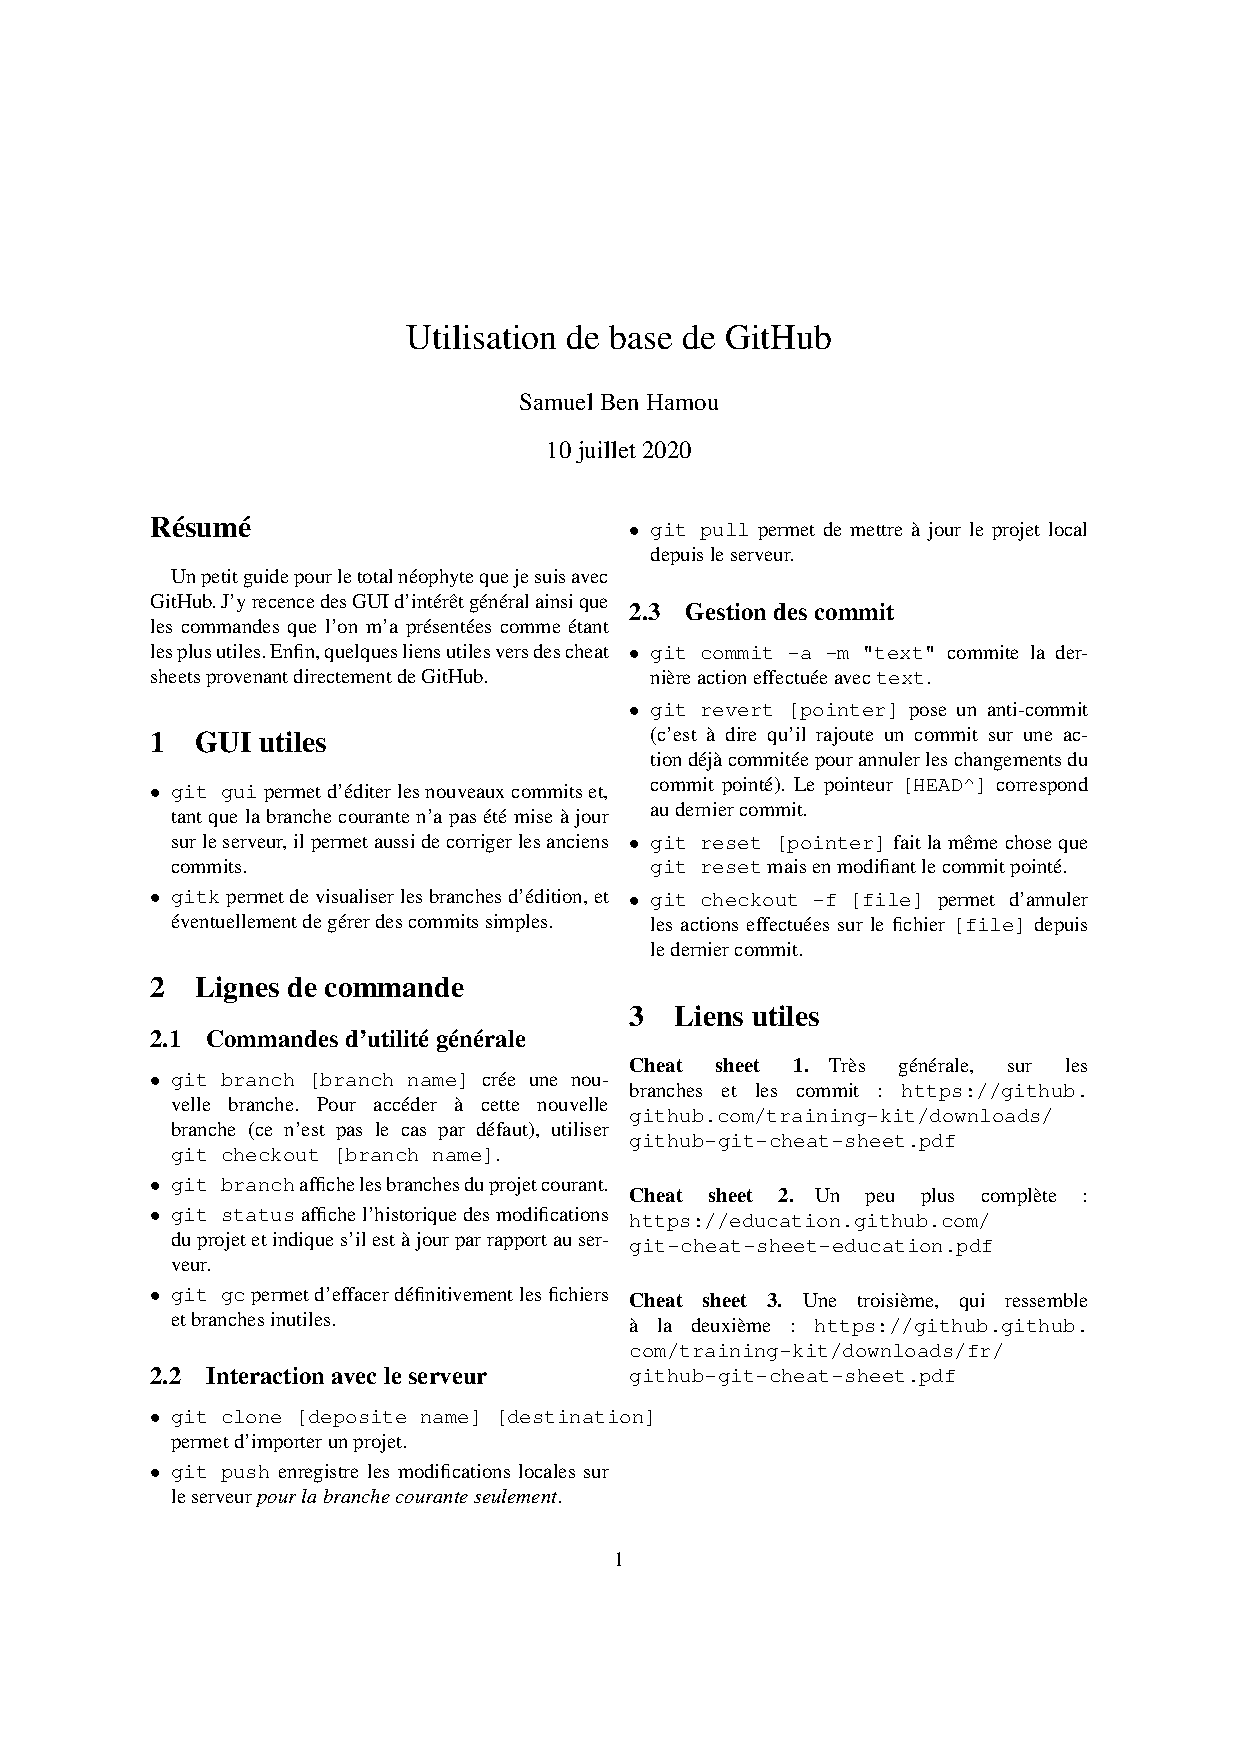
\includepdf[pages=1, nup=1x1, frame=true, scale=0.8, pagecommand=\section{Cheatsheet pour GitHub}\label{gitsheet}]{TutoGitHub.pdf}

\section{Commutativité de l'addition : avant-après}\label{beforeafter_comm_+}

\end{document}
